\section{Decision Tree}

% (全文指标和监控数据统一用metric表示,特征用feature表示,但是二者可以等同为同一个意思。在ML中称为feature,在AM中称为metric)

% 各种监控工具以及各种监控的数据,产生了许多指标数据,让GPU的性能分析变得异常复杂。Decision Tree可以利用信息理论筛选出最重要的指标集,更方便、快速地利用GPU架构的理论知识发现性能瓶颈并给出优化方案。

\subsection{Features and Hypothesis Space}

% 建立决策树模型的第一步需要形成特征体系。一个GPU microBenchmark可以形成一条记录,并且可以产生多种监控数据。
% 这些监控数据可以分为两类:一类与用户提交应用时指定的数据集、硬件固有属性等有关,例如输入数据集的大小,Global memory的带宽等;另一类是事实上反应了当前GPU架构和GPU应用架构下的运行特征,例如Global Memory的load/store数、L1 cache的命中率、Instruction的并行度等。
% 这两类数据都决定了一个GPU microBenchmark的运行结果,并且反映了一次运行的性能信息。
% 所以我们可以直接利用监控的metric作为一条记录的Feature。也就是说,一个metric就是一个feature。同时我们将用户指定或者硬件固有属性等不形容运行状态的Feature称为Static Feature(SF),而将形容运行状态Feature称为Runtime Feature(RF)。

% 在ML的特征工程中,除了监控可得的特征,还可以通过特征之间的非线性计算方法得到新的特征。例如,访问L1 cache的次数和访问Global memory的次数是两个特征,通过除法可以得到Global Memory的访问命中率,Global memory的访问命中率也可以作为一个新的特征。
% 传统的数学分析模型也提供了诸多的性能指标计算方法,这些都可以作为新的特征添加到特征体系中。我们将这种特征称为Assistant Feature(AF)。SF、RF和AF共同组成了GPU性能分析的特征体系。常用的特征值/指标值的含义及特征类型如表~\ref{table:metrics}所示。

Common examples of metrics (or features) used in this paper are shown in Table~\ref{table:metrics}.

\begin{table}[!t]
\small
%\lefting
\caption{Common Examples of Metrics/Features in this paper} 
\begin{tabular}{ l | l | l }
\hline
\textbf{Name} & \textbf{Metric Meaning} & \textbf{Type} \\
\hline
\textit{Input\_size} & size of input dataset & SF\\
\hline
\textit{TLP} & the thread level parallelism & RF \\
 \hline
\textit{ILP} & the instruction level parallelism & RF \\
\hline
\textit{SFU\_width} & width of special function units per SM & RF \\
\hline
\textit{Cache\_hit} & cache hit latency & RF \\
\hline
\textit{Sync\_over} & the overhead of waiting synchronization & AF \\
\hline
\end{tabular}
%\vspace{-4mm}
\label{table:metrics}
\end{table}

% 不可忽略的是在诸多的监控数据中存在具有一定关联性的特征值,因为往往一个性能瓶颈会影响多项类似的指标异常。例如数据放置不均衡,会导致L1 cache的load次数增加,同时必然导致Global memory的load次数增加,这两个特征值之间有一定的关联性。
% 这类关联特征往往一起影响GPU应用的运行状态,但是最终指向同一个关键因素,我们将这类特征/指标归结为一个特征集/指标集。在决策树模型中,每次决策选择当前最重要的特征,多次决策就可以得到一个特征集。在ML中,特征集之间的关联性往往会影响模型的准确性。但是我们后续基于特征集进行理论分析,不仅可以避免特征之间的关联性带来的模型的不准确性,还可以利用这个关联性定位性能瓶颈。

% 根据特征体系,我们可以得到用于决策的假设空间。假设空间可以确定特征值的有效性,决定是否能够建立决策树模型。要建立假设空间,必须考虑到每次监控的特征值不可能完全相同。因此,我们需要通过缩小监控值的精度,限定特征值的范围来建立假设空间。
% 分析GPU性能的Decision Tree的一个可能的假设空间如图~\ref{fig:hs}所示。假设空间的每一层都有一个关键的特征作为划分依据,根据特征的可能出现的值划分成多个数据集。

One possible hypothesis space of this paper is shown in Figure~\ref{fig:hs}.

\begin{figure}[!t]
\centering
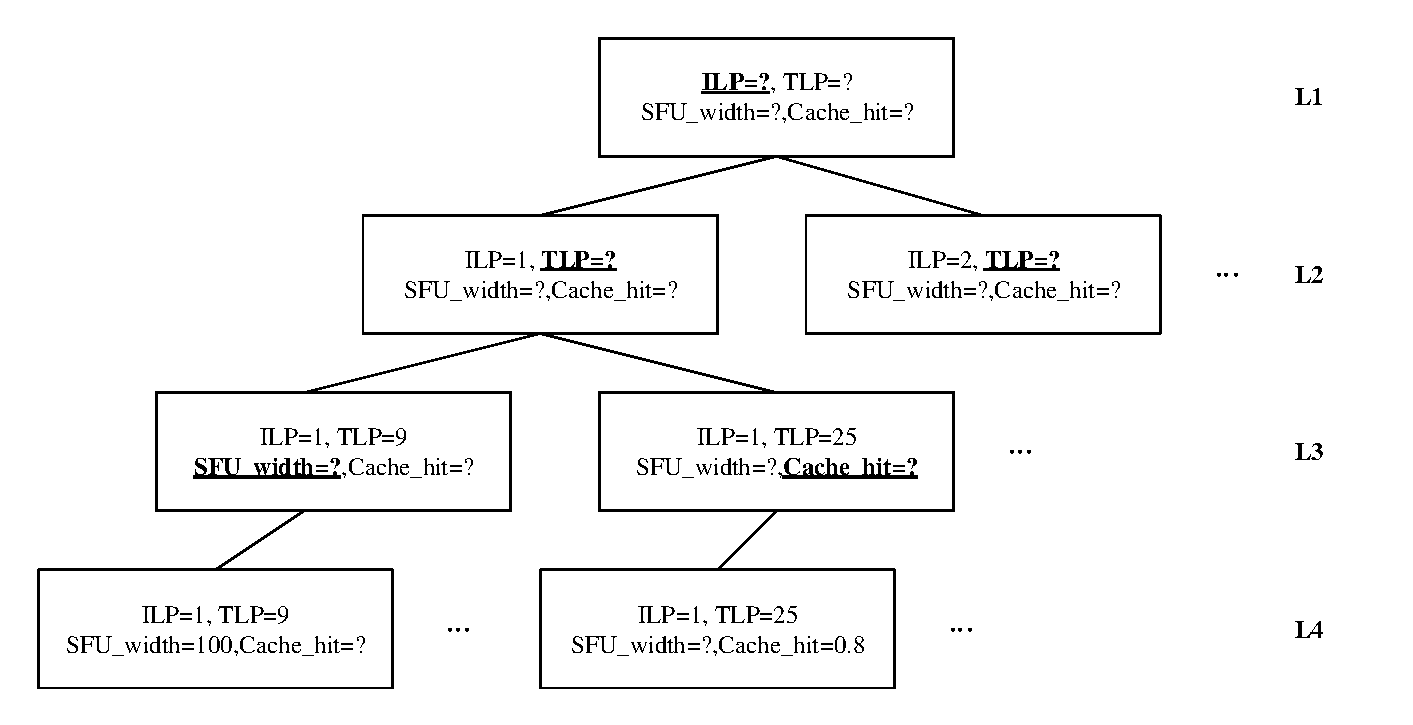
\includegraphics[width=0.5\textwidth]{hypothesisspace.pdf}
%\vspace{-2mm}
\caption{An Example of Hypothesis Space}
%\vspace{-4mm}
\label{fig:hs}
\end{figure}

\subsection{Training Set}

% (不建议每个应用跑几遍,否则会违背样本中“记录之间独立同分布”的默认特性,因此还是建议断点监测的方法。)

We choose these benchmarks to build the training set:

\begin{itemize}

\item micro-benchmarks

\item Pariol benchmarks.

\item Regal benchmarks.

\end{itemize}

\subsection{Decision Tree}
\label{subsec:decisiontree}

Decision Tree.

